

\section{Background} 
\label{sec:back}

In this project we were forced to investigate different ideas at three different research areas: heuristic based search, reinforcement learning and nature inspired algorithm. 
Of course there is an overlap between these approaches. All of them try to find the next best step for the agent by iterating through a search tree. This is build in base of all possible game steps that could done by the agent.
One naive approach of iterating through the whole search tree is not possible cause of the time limitation.
Generally this leads to find the trade-off between iterating similar to a breadth-first or depth-first search.
First of all we introduce an depth-first approach that uses an estimation function for looking many steps ahead.


\subsection{Heuristic Based Search} 

A \ac{HR} is used to evaluate a game state by putting several facts into one number. When we have to decide which current active branch of a search tree should be iterated this score might help us. 
One common idea to estimate the distance to the target is the manhatten distance~\cite{distance_metrics}. 

In a two dimensional space the manhatten distance is calculated by

\begin{equation}
dist(u,v) = |x_{1} - x_{2}| + |y_{1} - y_{2}|
\end{equation}

adding the absolute value of the difference for the $x$ and the $y$ axis. The input consists always of the points that have one value for each dimension. This could be extended for a n-dimensional space as well. When thinking of a way at a grid this is always a path with one rectangle waypoint (cf.~\cref{fig:manhatten}).

\begin{figure}
\centering
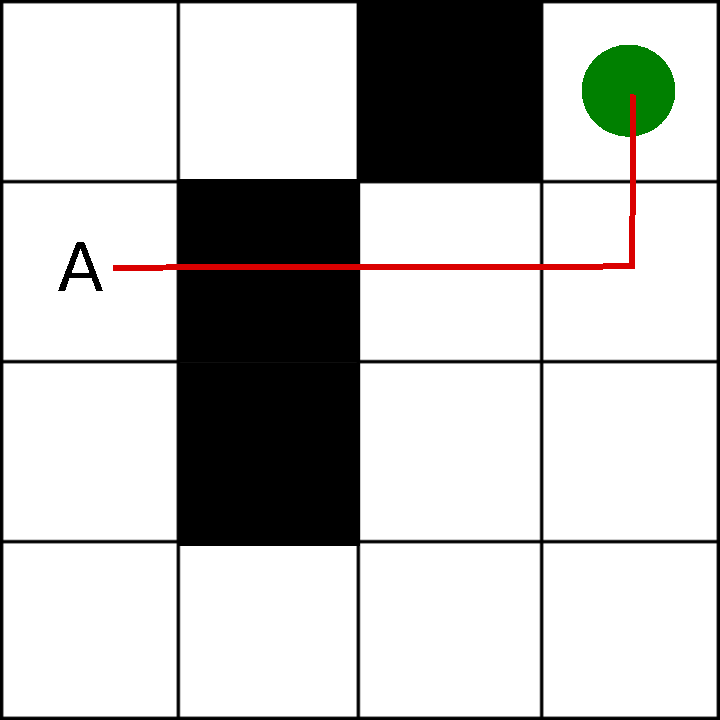
\includegraphics[scale=0.3]{images/manhatten.pdf}
\caption{Manhatten distance}
\label{fig:manhatten}
\end{figure}



\subsubsection{Greedy}

Greedy-algorithms are a whole class of algorithms and strategies. All of them follow a specific scheme/rule. They are iterative and choose in every step the state with the best reward. The state is in most cases a node which represents the state of the algorithm. The advantage of greedy algorithms is that they are very fast but on the other hand they are not optimal they often only find a local optima and not the global one. The advantage and disadvantage is caused by the greedy approach.  

\subsubsection{One Step Lookahead}

One step lookahead is a very simple tree search algorithm which follows the greedy approach. The actual state is the root node. From this node we only look one step ahead to all nodes which are connected by one edge and compute a heuristic value or another kind of reward value for these nodes (cf.~\cref{fig:onestep}). 

\begin{figure}
\centering
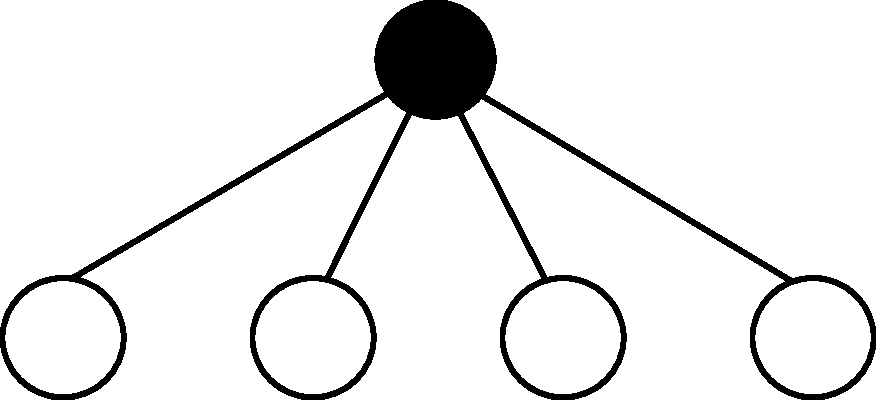
\includegraphics[scale=0.3]{images/onestep_lookahead.pdf}
\caption{Search tree for One Step Lookahead}
\label{fig:onestep}
\end{figure}


After that the algorithm terminates and we pick the node with the best heuristic value. This algorithm is a special greedy approach that
is limited by the first level at the search tree.

\subsubsection{AStar}

The A* tree search algorithm is a modification of the dijkstra algorithm and also belongs to the class of greedy algorithms. The Algorithm finds the shortest path between two nodes. In difference to normal greedy algorithms A* is a optimal algorithm, it finds a solution when a solution exists (in this case the shortest path). The algorithm uses a heuristic to estimate the shortest path. The value f(x) of a node N is the sum of its heuristic value h(x) and the costs from the start-node to N g(x).

\begin{equation}
f(x)=h(x)+g(x)
\end{equation}

\todo{any picture?}

A* contains two sets of nodes, the openlist and the closedlist. In every step of the algorithm the Node N with the lowest f(x) value in the openlist is put on the closedlist and all its connected nodes, which are not in the closedlist, are put in the openlist (with reference to their fahter N). If a connected node is already in the closedlist but the new generated value f'(x) is lower than f(x) then f(x) will be replaced by f'(x) and the new father-reference is N. The openlist contains all the nodes to which the path is already known and which can be checked in the next step, the closedlist contains every visited and checked node. When the actual node is the goal-node, the algorithm terminates. To generate the path, the algorithm goes back from the goal-node to the start node (guided by the father-references). 

\subsection{Reinforcement learning} 
 
\ac{RL} is a field in Machine learning which is a section of Artificial Intelligence. \ac{RL} methods are mostly used by agents in an environment called \ac{MDP}. \ac{MDP} is a mathematical description of decision processes. They have different states S and some actions A which are available in the actual state. Every timestep the agent chooses an action $a$ and the process switches from state $s_a$ to $s_n$. The probability to go over form a state S to another state S' by any action A can be described as

\begin{equation}
	G: S*S*A \rightarrow [0,1] 
\end{equation}

and the reward given to the agent can be described by this:

\begin{equation}
	R: S*S*A \rightarrow \mathbb{R}
\end{equation}

So that

\begin{equation}
	(s_a, s_n, a) \rightarrow p(s_n|s_a, a)
\end{equation}

would describe the probability $p$ to go over in the state $s_n$, given the actual state $s_a$ and the choosen action $a$ and 

\begin{equation}
	(s_a, s_n, a) \rightarrow r
\end{equation}

shows its corresponding reward.  


In differ to other learn methods and approaches like the (semi)supervised learning, RL algorithms never use information which they do not figured out themselves, so no correct samples were given to the algorithm. The only information is the reward given to the agent and some additional information like heuristic values, depending of the specific algorithm. 
A big problem problem in \ac{RL} is the conflict between exploration of new and unvisited areas of the solution room and exploitation which is the improvement of already found solutions.
...
\subsubsection{Monte Carlo Tree Search} 

\ac{MCTS} is a class of \ac{RL} algorithms. It is the most important concept in this paper. \ac{MCTS} needs a tree of nodes which represent the different states, the edges represent the actions used by the agent to get to this node. The \ac{MCTS} algorithm traverses to this tree and expands it. To find the global optimum a good balancing ratio between exploration and exploitation is required. 

\todo{[maybe picture from his paper and pseudocode, wird vielleicht zu viel...]}


The general \ac{MCTS} algorithm has four steps, selection, expansion, simulation and backpropagation.
In the selection the algorithm starts at the root node and traverses down the tree. Goal of this step is to select a node to expand (to generate a child node). Depending on the number of children of every node there are several different paths we can chose. Often the $Upper Confidence Bound for Trees$, (UCT) is used to balance the ratio between expolitation and exploration:
\begin{equation}
	UCT = \overline{X}_j + 2 * C * \sqrt{\frac{2 \ln n}{n_j}}
\end{equation}
$\overline{X}_j$ is the average reward of this node so the left part of the formula is the exploitation part. The right part generates the value for exploration, where $C$ is a constant (often $\sqrt{2}$), $n$ is the number of times the parent node has been visited and $n_j$ is the number of times the actual node was visited.This formula has shown to provide good resultsand it is part of a lot of \ac{MCTS} algorithms.
After the selection of a node one randomly chosen child is generated, this is called the expansion.
The third step is the simulation in which we want to know how good the extended node is. To do that, we generate randomly chosen children from the expanded node. When we reach our simualtion depth we compute the reward of the last simulated node.
In the last step, the backpropagation, we start at the expanded node and iterate to the root, guided by the father references. In every node we visit the reward of the simulation will be charged with the actual reward of the node.
The first two steps are guided by the so called Tree Policy, the simulation by the Default Policy.
\todo{maybe more detailed -> but the chapter will be very large}

\subsection{Nature inspired} 
The nature is solving problems by applying different approaches instinctively. Computer scientists used that observed knowledge from the
nature to write \ac{NI} algorithms that has a similar procedure. Our brain could solve problems that could not be solved by an algorithm until now. Funnily this is often the truth for games for example poker.

\subsubsection{Neural nets} 
Many researcher try to explore the process of the human brain. Neural networks tries to model the nervous system and to adapt all the processes~\cite{nn_intro}. The neurons are modeled as \ac{TLU} that consists of several input values $x_1$ to $x_n$ and one output value $y$~\cite{ci_kruse}. 


\begin{figure}
\centering
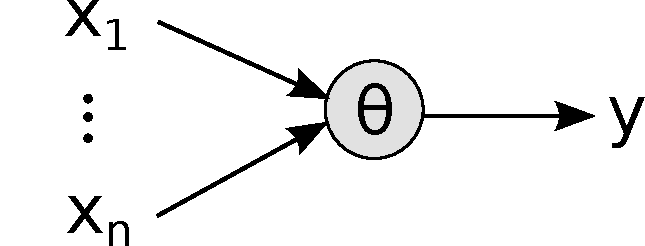
\includegraphics[scale=0.5]{images/tlu.pdf}
\caption{\ac{TLU}~\cite{ci_kruse}}
\label{fig:tlu}
\end{figure}


For computing the output value is always for every input value one weight $w_i$ and the threshold $\theta$. The formula 

\begin{equation}
    y = 
\begin{dcases}
    1, & \text{if } \sum_{i=1}^n w_{i} x_{i} \geq \theta \text{,} \\
    0, & \text{otherwise.}
\end{dcases}
\end{equation}

is used to calculate the output $y$ that is either 0 or 1.
Normally the weights are learned by a given input and output. With only one \ac{TLU} only linear separable spaces could be learned perfectly.
To solve that problem there is the possibility to create a network of \acp{TLU} and map that problem to a higher dimensional space~\cite{ci_kruse}.


\subsubsection{Evolutionary algorithm} 
An \ac{EA} tries to use the biological behavior of the population~\cite{evo}. 
This algorithms follow two main ideas. Firstly there are operators like the recombination (crossover) or
mutation that allows to create different individuals. Secondly every iteration is a selection to guarantee
a good quality.
The procedure is shown at the~\cref{alg:evo}. 


\begin{algorithm}
\caption{Evolutionary Algorithm~\cite{evo}}
\label{alg:evo}
\begin{algorithmic}
\State \emph{Initialize} Population with random candidate solutions;
\State \emph{Evaluate} each candidate;
\While{Termination condition not satisfied} 
\State \emph{Select} parents;
\State \emph{Recombine} pairs of parents;
\State \emph{Mutate} the resulting offspring;
\State \emph{Evaluate} new candidates;
\State \emph{Select} individuals for the next generation;
\EndWhile
\end{algorithmic}
\end{algorithm}

First of all there is the initialization phase to create a pool with random
individuals. After that the score of each of them has to be evaluated. Often there
is a problem for optimization problems with a fast evaluation. This duration is
strictly linked with the duration of the whole algorithm.

The while loop needs to have a termination condition. On the one hand this could be
a predefined score that the best individual in one generation could have. On the other 
hand it could be a time limit that should not be exceeded.
Every iterations starts with a selection of the parents.
These are used to create new individuals by performing crossovers and mutations.
The challenge is made of finding good functions for that operations. 
Since the pool size is limit there is a selection of the fittest in every iteration.

Often evolutionary algorithms are used for optimization problems because there
hopefully better than a random search.

